% 
% Licensed to the Apache Software Foundation (ASF) under one
% or more contributor license agreements.  See the NOTICE file
% distributed with this work for additional information
% regarding copyright ownership.  The ASF licenses this file
% to you under the Apache License, Version 2.0 (the
% "License"); you may not use this file except in compliance
% with the License.  You may obtain a copy of the License at
% 
%   http://www.apache.org/licenses/LICENSE-2.0
% 
% Unless required by applicable law or agreed to in writing,
% software distributed under the License is distributed on an
% "AS IS" BASIS, WITHOUT WARRANTIES OR CONDITIONS OF ANY
% KIND, either express or implied.  See the License for the
% specific language governing permissions and limitations
% under the License.
% 

\section{Reservations Page}
\label{sec:ws-reservations}

This page shows details of all reservations.  There are two types of reservations: {\em managed}
and {\em unmanaged}.

A {\em managed reservation} is a reservation whose process is fully managed by {\DUCC}.  This process
is any arbitrary process and is submitted with the
\hyperref[sec:cli.ducc-process-submit]{ducc\_process\_submit} CLI.  The lifetime of the reservation
starts at the time {\DUCC} assigns a unique ID, and ends when the process terminates for any reason.

An {\em unmanaged reservation} is essentially a sandbox for the user.  {\DUCC} starts no processes
in the reservation and manages none of the processes which run on that host.  The lifetime of the
reservation starts at the time {\DUCC} assigns a unique ID, and ends when the submitter or system
administrator cancels it.

The Reservations page contains the following columns: 
\begin{description}

\item[Id] \hfill \\
  This is the unique {\DUCC} numeric id of the reservation as assigned when the reservation is made.
  If this is a {\em managed} reservation, the ID is hyperlinked to a
  \hyperref[sec:ws-managed-reservation-details]{Managed Reservation Details} page with extended
  details on the process running in the reservation.

\item[Start] \hfill \\
  This is the time the reservation was made.
  
\item[Duration] \hfill \\
  A time in green is the length of time the active reservation has been assigned.  
  A time in black is the length of time the completed reservation was assigned. 
  
\item[User] \hfill \\
  This is the userid that made the reservation.
  
\item[Class] \hfill \\
  This is the scheduling class used to schedule the reservation.
  
\item[Type] \hfill \\
  This is the reservation type, {\em managed} or {\em unmanaged}, as described 
  \hyperref[sec:ws-reservations]{above}.

\item[State] \hfill \\
  % 1. org.apache.uima.ducc.transport.event.common.IDuccState
  This is the status of the reservation. Values include: Received - Reservation
  has been vetted, persisted, and assigned unique Id.
  \begin{description}
  \item[Assigned] - The reservation is active. 
  \item[Completed] - The reservation has been terminated.
  \item[Received] - The Reservation has been vetted, persisted, and assigned a unique ID.
  \item[WaitingForResources] - The reservation is waiting for the Resource Manager to find and 
    schedule resources. 
  \end{description}

\item[Reason] \hfill \\

  % 2. org.apache.uima.ducc.transport.event.common.IDuccCompletionType

  If a reservation is not active, this shows the reason.  Note that for
  {\em unmanaged reservations}, even if the user has processes running in the
  reservation, {\DUCC} does NOT attempt to terminate those processes (hence, ``unmanaged''.)

  For {\em managed reservations}, {\DUCC} does terminate the associated process.

  \begin{description}
  \item[CanceledBySystem] - In the case of the special JobDriver reservation, this is
    canceled by {\DUCC} and reestablished on reboot; hence the state is a result of {\DUCC}
    having been restarted.

    In all other cases, it is a result of {\DUCC} being restarted {\em COLD}.  When
    {\DUCC} is started {\em COLD}, all previous reservations are canceled.  (When {\DUCC}
    is started {\em WARM}, the default, previous reservations are preserved.)
  \item[CanceledByAdmin] - The {\DUCC} administrator released the reservation. 
  \item[CanceledByUser] - The reservation owner released the reservation. 
  \item[ResourcesUnavailable] - The Resource Manager was unable to find free or freeable resources 
    to match the resource request. 
  \item[ProgramExit] - The reservation is a {\em managed} reservation and the associated
    process has exited.
  \end{description}

\item[User Processes] This is the number of processes owned by the user running in the reservation.  
  
  Note that even for {\em unmanaged} reservations, the {\DUCC} agent tracks processes owned
  by the user and reports on them.  This allows better identification and management of
  abandoned reservations.
          
\item[PgIn] This is the number of page-in events for the managed reservation.

\item[Swap] This is the total swap space for the managed reservation.

\item[Memory] \hfill \\
  The memory size in GB of the reservation.  This is the amount of memory that
  was {\em requested}.  In the case of RESERVE policy reservations, that actual memory
  of the reserved machine may be greater.
  
\item[Host Names] \hfill \\
  The host names of the machines where the resources are allocated.
  
\item[Description] \hfill \\
  This is the description string from the --description string from submit.
\end{description}

    \begin{figure}[ht!]
    \centering
    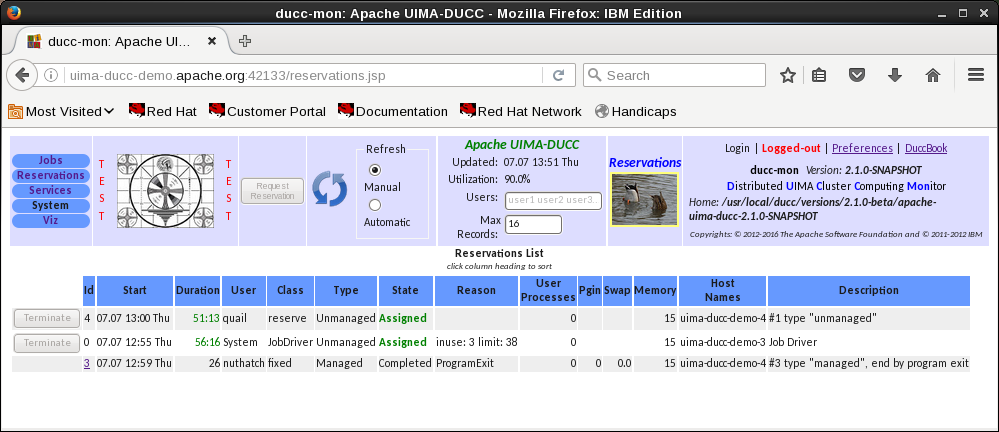
\includegraphics[width=90mm]{images/ducc-webserver/Reservations.png}
    \caption{Reservations Page}
    \end{figure}
